\chapter{Modeling, sculpting and UVs}
\label{ch:model}

\section{Edit Mode}
\key{Tab} enters Edit Mode; \key{1} / \key{2} / \key{3} pick vertex, edge and face selection. The tools follow the
selection mode, as in ProBuilder and Blender:

\begin{center}
\begin{tabularx}{\textwidth}{llX}
\toprule
Do & Unity keymap & What it does \\
\midrule
Extrude & Ctrl+E & pull new geometry out of the selection; a lone vertex grows an edge, an edge a face \\
Inset & I / Ctrl+I & a smaller face inside each face (or the selection as one region) \\
Bevel & Ctrl+B (wheel: segments) & round or chamfer edges, with a profile from concave to convex \\
Loop cut & Ctrl+R over an edge & cut a ring of new edges round the mesh \\
Knife / Line & K & split a face between two points with endpoint, midpoint and on-edge snapping \\
Bridge & Ctrl+Shift+B & join two faces or two holes with a tube \\
Merge at center / Fill & Alt+M / Alt+F & collapse vertices, close holes (Smart Fill on open loops) \\
Dissolve / Connect & Ctrl+X / J & remove edges keeping the surface; cut between two vertices \\
Select loop / ring & Alt+click / Ctrl+Alt+click & edge loops and rings; face loops in face mode \\
Push/Pull / Push Through & P / Alt+P & SketchUp's face operator; a hole along the normal \\
\bottomrule
\end{tabularx}
\end{center}

Every modal operator behaves the same way: start with the key; move the mouse or type a number (\key{X} / \key{Y} /
\key{Z} lock an axis, twice for the local axis; \key{Shift}+axis locks a plane; \key{Ctrl} snaps; \key{Shift} is fine
control; during a bevel the wheel sets the segments, or \key{]} / \key{[} without one); a click or \key{Enter} confirms;
\key{Esc} or a right-click cancels leaving no undo step; then \textbf{Adjust Last Operation} (\key{F9}) changes the
values afterwards as the same step and remembers them as the tool's defaults. A hint bar at the bottom of the Scene
view lists the keys while any of them runs. \textbf{Proportional editing} (\key{O}) moves nearby vertices with a falloff.
\textbf{N-gon Mode} treats each flat region as one face, as SketchUp does. Shift+drag a gizmo handle extrudes first.

\textbf{Modifiers} stack non-destructively, top to bottom, as in Blender: Array (with Fit Length / Fit Curve), Bevel,
Boolean, Decimate, Mirror, Screw, Solidify, Subdivision Surface \cite{Catmull1978Recursively}, Triangulate,
Wireframe, Weld; and the deformers Cast, Curve, Displace, Lattice, Mesh Deform, Simple Deform and Smooth. Each has
Edit Mode / Viewport / Render toggles and a header as Blender's; drag a modifier's name to move it; Apply works on one
modifier ignoring those above it. \textbf{Curves and lattices}: \menu{GameObject > Curve} makes Bezier, circle and path
curves; a Lattice is a box of points that squashes the mesh inside it; their points take the same keys as vertices.

\textbf{Checks.} Select Overlapping and the Z-fighting check find faces on top of each other; Delete Loose removes stray
vertices; Recalculate Normals (\key{Shift+N}) faces everything outwards; Auto Smooth shades by angle; Select Similar
and Select by Material; \menu{Mesh > From Papers} has the tools built from research papers (Taubin smoothing
\cite{Taubin1995Signal} and others).

\begin{example}{a rounded table top}
\begin{enumerate}
  \item Create a Cube, scale it to 1.6 $\times$ 0.05 $\times$ 0.9.
  \item \key{Tab} into Edit Mode, \key{2} for edges, \key{Ctrl+Alt}+click one of the four vertical edges (an edge ring).
  \item \key{Ctrl+B} and drag; scroll for segments. \key{F9} to set the width exactly.
\end{enumerate}
\end{example}

\section{Sculpting}
\menu{Modeling Tools > Sculpt} (\code{sculpt on}) is ZBrush's workflow on the mesh under the pen \cite{ZBrushDocs2026}:
brushes (Clay Buildup, Draw, Inflate, Smooth, Grab, Snake Hook, Crease, Flatten, Scrape, Pinch) with Mirror symmetry
and Radial, a lazy mouse, image alphas and stroke types (Dots, Drag Dot, Drag Rect, Freehand, Spray); masks (\key{Ctrl}
paints, \key{Ctrl+I} inverts) that keep a brush off a region; polygroups in the eight colour-universal colours
\cite{Okabe2008Color} and hiding (\key{H} / \key{Alt+H}) to work on a part alone; a stroke one light undo step; the
pen's pressure, tilt and eraser end (the \key{[} / \key{]} keys step the size). Four ways to add resolution:
\textbf{Dynamic Subdivision} (a Catmull--Clark preview the brush edits through; the base mesh stays light),
\textbf{DynaMesh} (the shell retopologized evenly from its winding number \cite{Jacobson2013Robust,
Gibson1998Constrained}; two shapes merged into one skin), \textbf{Quad Remesh} (QuadriFlow \cite{Huang2018Quadriflow}
on a worker: a clean quad mesh at a target count, with Blender's Eigen) and \textbf{Dyntopo} (Sculptris Pro
\cite{SculptrisDocs2026}: the mesh tessellated under the brush as it moves). The pipeline order that keeps a model
clean: \emph{sculpt $>$ remesh $>$ unwrap $>$ bake mesh maps $>$ paint}; a remesh after painting would throw the paint's
UVs away.

\section{UV unwrapping}
Layout $>$ UV Unwrapping puts the \textbf{UV Editor} (\key{Ctrl+9}) beside the Scene view.
\begin{enumerate}
  \item In Edit Mode select the edges where the mesh should be cut open and \ui{Mark Seam} (or UV $>$ Seams from Sharp
    Edges).
  \item Select everything and press \key{U} to Unwrap (LSCM, as Blender's \cite{Levy2002Least}). \ui{Smart UV} projects
    by angle; \ui{Part Unwrap} finds charts by parts with ABF++ \cite{Sheffer2005Abf, Wang2025Partuv}; cube, cylinder,
    sphere and view projections are there too.
  \item In the UV Editor move, rotate and scale islands with the gizmo (\key{W} / \key{E} / \key{R}); \ui{Pack} fits them in
    the square; \ui{Avg Scale} evens them; the \ui{Stretch} overlay shows where a texture would distort; \ui{Sync} sets
    Edit Mode's faces from the UV selection. After Unwrap, Smart UV or Pack, \key{F9} changes the margin.
\end{enumerate}

\begin{figure}[H]
  \centering
  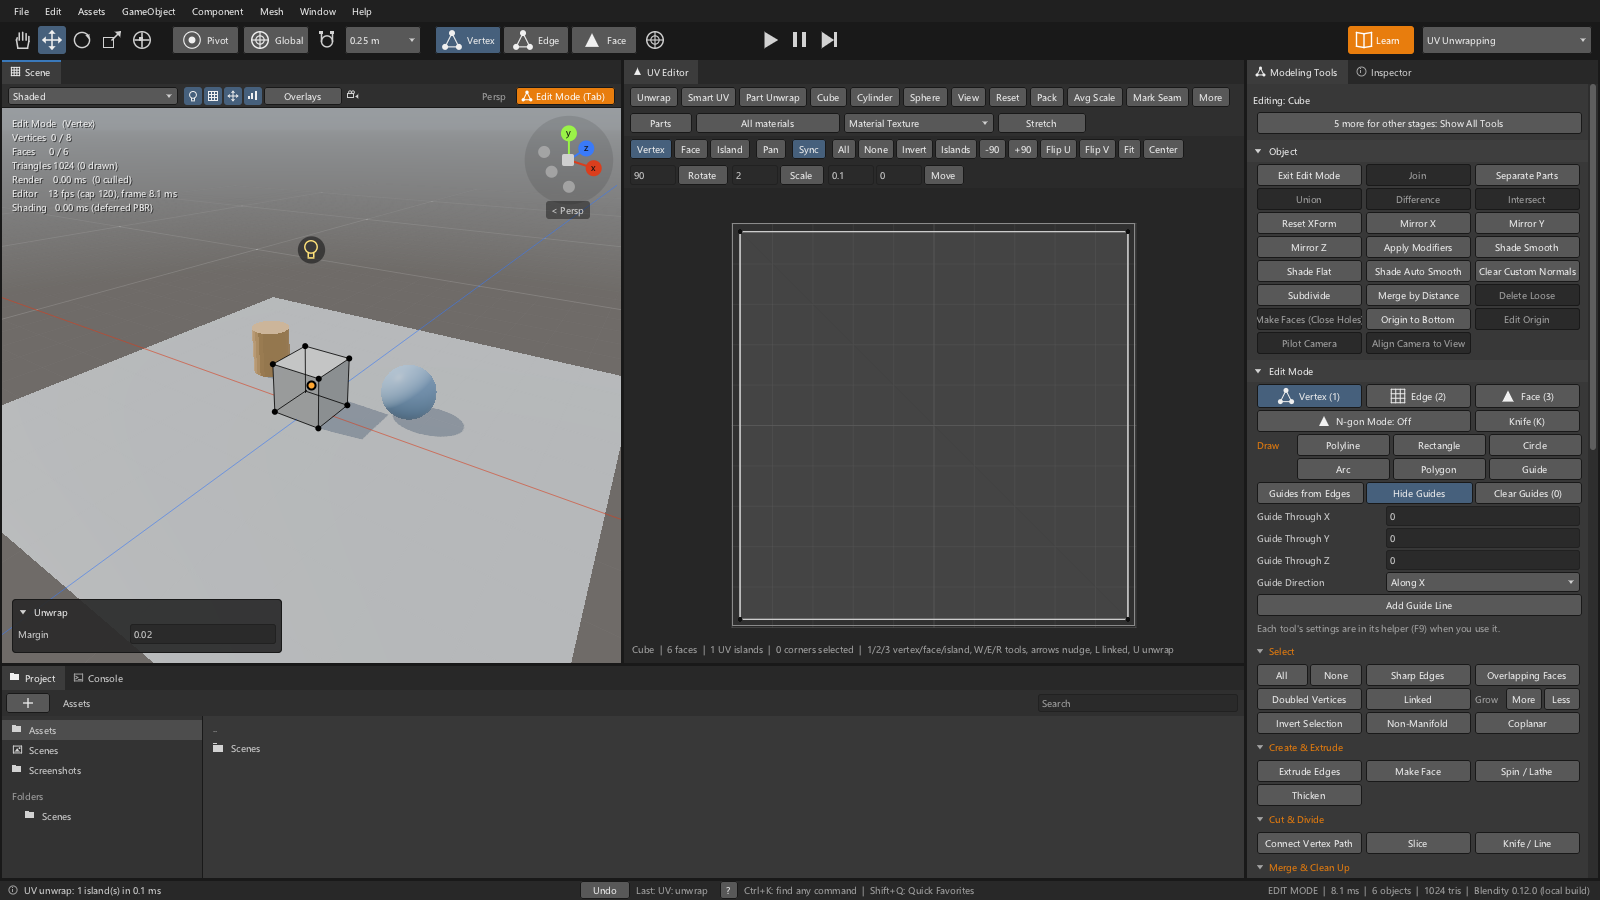
\includegraphics[width=\textwidth, alt={The UV Unwrapping layout: the Scene view with a cube in Edit Mode on the left, the UV Editor with its toolbar and the unwrapped cube's islands in the middle, the Modeling Tools window on the right.}]{layout-uv.png}
  \caption{The UV Unwrapping layout: Edit Mode on the cube, the UV Editor's toolbar (Unwrap, Smart UV, Part Unwrap, the
  projections, Pack, Mark Seam; vertex / face / island selection; the transforms) and the Modeling Tools beside it.}
\end{figure}

\begin{example}{a crate with a clean texture layout}
\begin{enumerate}
  \item Create a Cube; Edit Mode, select all, UV $>$ Cube Projection.
  \item Set the UV Editor's background to UV Grid (Blender's test image) to check that the squares stay square.
\end{enumerate}
\end{example}

\begin{fromnote}{Where it comes from}
Edit Mode's operators follow Blender's BMesh operators and editors
\cite{Blender2026, BlenderManual2026}; Push/Pull, inference and Follow are SketchUp's \cite{SketchUpHelp2026}; Follow,
Lathe and Slice are UModeler's \cite{UModelerDocs2026}; Shell, Draft, Radial Array and the construction planes are
Plasticity's \cite{PlasticityDocs2026}; the parametric shapes are ProBuilder's \cite{ProBuilderDocs2026}; the sculpt
brushes, masks and remeshers follow ZBrush and Sculptris \cite{ZBrushDocs2026, SculptrisDocs2026}; the theory is in
\cite{MarschnerShirley2021} (meshes, texture coordinates). Learn: \emph{Meshes: Vertices, Edges, Faces}, \emph{Edit
Mode: Modeling Like Blender}, \emph{Modifiers vs Components}, \emph{Advanced Modeling Tools}, \emph{Bevel, Bridge and
Push Through}, \emph{Sculpting}, \emph{UV Mapping}.
\end{fromnote}
